
\section{Background}

% ---------------------------------------------- %
% Temporary working notes                        %
% ---------------------------------------------- %
%
% traditional noise (need not be explained in detail):
%   * ring artifacts
%   * salt/pepper noise
%
% distortion (explained a bit more):
%   * beam hardening
%   * refration on implant
%   * scattering effects
%
% formørkning (ydre kant af implantat)
% forlysning (overflade af implantat)
%
% Phantom image of implant in air can be explained briefly
%
% red-yellow-blue colormap has been used
%   - red = 0
%   - soft yellow = 128
%   - blue = 255
% -but intensities are inverted in regards to absorption !
% ---------------------------------------------- %

\subsection{The physical samples}

The physical samples are prepared for SR$\mu$CT scanning by cutting out a portion of a larger
12mm cylindrical sample. \aleksandar{Better to give a brief chronological tour of how the sample has been handled? Time scale also matters to mention in regards to growth.} The cut samples are 6.5mm cubes \aleksandar{more accurate measures?}. This contains the titanium dental implant (Astra Tech OsseoSpeed, ST Molndal, Sweden), which is 3.5mm in diameter and 8mm long. Along its length the lower 5.5mm has larger threads and is attached to recipient bone. The upper 2.5mm has smaller threads and is where newly formed bone is to be assessed. Sorrounding the bone and implant contact-region are cavities containing resin, air, blood vessels and other fibrous tissue. This is shown in figure \ref{fig:3viewsample}.

\begin{figure}%[!t]
\centering
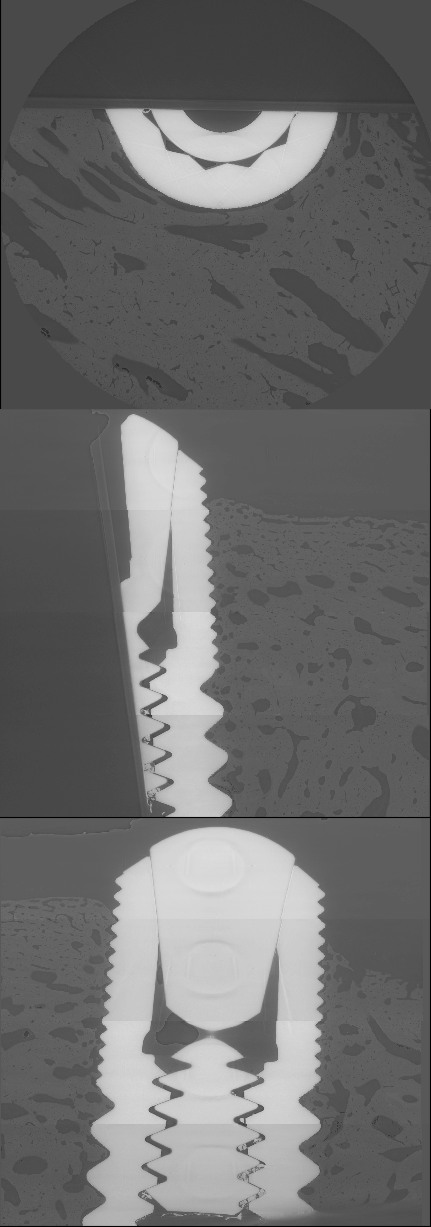
\includegraphics[scale=0.50]{figures/3_view_sample.png}
\caption{\aleksandar{Temporary example figure of sample in x,y,z dimension. It could perhaps even be manually annotated (meaning we can indicate roughly what regions correspond to: resin, air, implant, bone), and related to the physical scale mentioned above? Maybe as simple as overlaying a ruler with the given scale?}}
\label{fig:3viewsample}
\end{figure}

Each material has a different density and thus absorption. The titanium implant has higher absorption than bone.
Bone material then has higher absorption than its sorrounding tissue, vessels, air and resin.

\subsection{Data acquisition}

It can be difficult to study and evaluate the bone structure and blood network without destroying or
manipulating the sample. X-ray computed tomography is a widely used tool for non-intrusive medical
imaging. By exposing a subject to X-rays, we can map the linear attentuation coffecient of the passing
rays. Each ray is attenuated relatively to the density and composition of the material it passes. By
rotating either the scanner or the sample we can get a full 3D image representation of the inner
structure of the sample. Each volumetric pixel (voxel) then represents the X-ray attenuation at its spatial position. We can therefore reliably use X-rays to internally characterise samples in a non-intrusive and non-destructive manner. Regular CT-scans can provide spatial resolutions on the order of millimetre scale.\aleksandar{ref} The more modern micro computed tomography ($\mu$CT) can provide much higher spatial resolution on the micrometre scale.\aleksandar{ref} Both setups utilize poly-energetic beams, which can cause artifacts around high density regions. This effect is called beam-hardening\aleksandar{ref}, and occurs when rays with lower energy are attenuated more frequently. This offsets the local contrast, by overestimating the attenuation, leaving lighter spots on the image. Many other types of artifacts will also occur in these common scanners, but most is taken into account by calibration using phantoms and pre-hardening the beam before it reaches the sample. Due to its common usage, much software also exists to correct for noise and smaller imperfections during reconstruction\aleksandar{ref}.

This work focuses on data acquired by Synchrotron Radiation micro-CT (SR$\mu$CT). For this imaging
technique, electrons are accelerated to ultra-relativistic speeds in trajectories directed by strong
magnetic fields. Contrary to both CT and $\mu$CT, this approach requires a large particle accelerator, and is not standard medical or laboratory equipment\aleksandar{ref}. The added complexity means that SR$\mu$CT can offer an even better spatial resolution of up to 0.1 $\mu$m. The resulting beams are high in brilliance and collimation which gives a very clear signal. Its mono-energetic nature also means that images are not subject to artifacts from beam-hardening.

\aleksandar{Can we confirm whether data was acquired at the ESRF and at which beamline? Also which energies were used? All this could be important for reproducibility.}

\aleksandar{Was filtered backprojection used to do reconstruction, and who has done that? Was it done at ESRF?}

\subsection{Image data}

A single image sample contains voxels with of spatial resolution 1.875$\mu$m. The physical size of
a sample is about 6.5mm, which makes the raw dimensions of a single image $(3480,3480,3384)$ pixels.
For computational purposes, this has been cropped to be divisible by $2^5=32$. A full image sample
is further split into 4-6 sub-volumes through the height of the implant. This gives a size of $(3456,3456,810)$ pixels per sub-volume, where the last axis gets stacked for a full volume.

\aleksandar{OBS: 846 i rå størelse, 810 er efter volume-matching.}

\aleksandar{Important to explain a bit about how the samples were cut during acquisition. How were the samples secured in order not to be shifted too much etc.}

\subsection{Physical effects, noise and artifacts}

Noise in tomography is unavoidable, and it makes segmentation harder. Matarials may be well separated from certain angles in the 3d-reconstructed image, but overlap from others. Some noise like that corrected by flat-field correction is very uniformly distributed across images. Some noise is however very spatially dependent on its sorrounding regions. Since we know the compositions of the materials being imaged, we can counter some of these effects during segmentation. The noise effects manifest themselves as numerical shifts in voxel-values as a function of their position. This is a direct result of a misrepresented attenuation along the axis the X-rays are passing. 

\aleksandar{perhaps we should mention at what energies the data is taken. This helps to narrow which types of effects play into the data.}

Low energy rays contribute mostly with noise from scattering effects. A ray will propagate through a material, get scattered and diffract from its initial trajectory. This gives a misrepresentation of the attenuation along its initial trajectory.

Streaking artifacts from dense implant region, but also in the transition from bone to softer tissue.

...

For SR$\mu$CT a high photon flux allows for very short exposure times \citep{srexptime}.
This can help counter noise from suboptimal counting statistics\citep{srnoise}.


* Gå fra brede effekter som viser sig i hele billedet (og er mere generelle) -> Til de mere specifikke effekter som er mere specifikke for vores case

* genskær fra voxels
mørke effekter modsat lysere effekter fra beam-hardening (x-rays er inverteret)

Forklare hvorfor vi ser mørke områder, særligt at det mørke lægger sig omkring implantatet,
men at det så aftager mod knoglen, for så at blive kraftigere og bredere helt ved knoglen..
nok refraktion osv. \aleksandar{OBS: before talking about specific noise in our data, we should probably include one or more examples of noise that shows how the segmentation is made harder due to this noise.}

% -------------------------------------------------------------------------------- %

\section{For Carl to include in method}

In figure \ref{fig:flowchart} we see a simple overview of the whole process.
  
\begin{figure}[!h]
\centering
\begin{tikzpicture}[>=latex']
        \tikzset{block/.style= {draw, rectangle, align=center, minimum width=2cm,
                                minimum height=1cm,draw=black,fill=gray!20, solid,
                                inner sep=0.25cm}}
               
        \node[block]                (box0) {Field computation (EDT + Diffusion)};
        \node[block, below=of box0] (box1) {2D-histograms (from fields)};
        \node[block, below=of box1] (box2) {Curves for material identification};
        \node[block, below=of box2] (box3) {Probabilities};
        \node[block, below=of box3] (box4) {Segmentation};

        \path[draw,->,thick] (box0) edge[line width=0.5mm] (box1)
                             (box1) edge[line width=0.5mm] (box2)
        				     (box2) edge[line width=0.5mm] (box3)
        					 (box3) edge[line width=0.5mm] (box4)
                             ;
\end{tikzpicture}
\caption{Flowchart caption goes here.}
\label{fig:flowchart}
\end{figure}
